\documentclass[UTF8]{article}
\usepackage{ctex}
\usepackage{amsmath}
\usepackage{graphicx}

\begin{document}
\section{机械波}
\subsection{机械波的基本属性}

    一、波的定义:波是自然界中一种常见的物质运动形式,波仅伴随着加载信息的能量传递

    质点运动:实体载着信息和能量运动,若干包含能量的小的物质集合的整体运动

    波的传播:信息和能量的传播,没有物质实体的移动,能量的扩展分布,充满其传播空间

    二、波的分类:

    1.机械波:机械振动在弹性介质中的传播,在介质中传播时受牛顿定律的支配

    2.电磁波:可以在真空中传播

    3.物质波:微观粒子具有波动性,反应概率密度的空间分布

    波的共同属性:都伴随能量传播,有反射、折射、干涉、衍射现象

    三、机械波的基本属性:机械振动(波源)在弹性介质(通过相互之间的弹性力组合在一起的连续介质)中的传播形成机械波。
    
    机械波产生条件:振源+弹性介质

    是运动状态的传播,弹性介质的质点并不随波传播.
    
    四、横波和纵波

    1.横波:质点振动方向与波的传播方向相垂直的波。特征:具有交替出现的波峰和波谷;仅在固体中传播

    2.纵波:质点振动方向与波的传播方向相平行的波。固、液、气体中均可传播

    横波和纵波都是行波

\subsection{机械波的描述}

    一、波线和波面

    波面:某时刻,同一波源向外传播的波到达的空间各点连成的面(同相位面)
    
    波阵面:波在传播过程中行进在最前面的波面,又称波前

    波(射)线:描述波传播的方向的射线。在各向均匀介质中波射线垂直于波面,波射线是波的能量传播方向

    根据波面的形状,可以将波分为:球面波(点源)、柱面波(线源)、平面波(面源)

    二、波函数与波动曲线

    波形图:$y = y(x,t)$,某时刻各点振动的位移y(广义:任一物理量)与相应的平衡位置坐标x的关系曲线

    三、机械波的特征量

    振幅:A\;\;质点偏离自身平衡位置所达到的最大正向位移

    波长:$\lambda$\;\;一个完整波形的长度。即:沿波的传播方向,两个相邻的、相位差为$2\pi$的振动质点之间的距离

    周期:T\;\;波前进一个波长的距离所需要的时间

    频率:单位时间内波动所传播的完整波的数目,$\nu = \frac{1}{T}$

    周期或频率只决定于波源的振动

    波速:u\;\;波动过程中,某一振动状态(即振动相位)单位时间内所传播的距离(相速)

    \[u = \frac{\lambda}{T} = \lambda\nu]\;\;\;\lambda = \frac{u}{\nu} = Tu\]

    波速只决定于媒质的性质

    固体内:横波\;$u = \sqrt{\frac{G}{\rho}}$,纵波\;$u = \sqcup\frac{E}{\rho}$

    液体、气体内:纵波\;$u = \sqrt{\frac{K}{\rho}}$

\subsection{平面间谐波波函数}

    一、平面间谐波

    1.平面简谐波定义:平面波传播过程中,若介质中各质元均做同振幅、同频率的简谐振动,该波称为平面简谐波

    2.平面简谐波产生条件:作简谐运动的波源\;+\;均匀无吸收的弹性介质

    3.平面简谐波是最基本、最简单的波动形式,复杂波可看成是不同频率简谐波叠加的结果

    二、平面简谐波波函数

    反映平面简谐波在均匀介质中传播时,介质中各质元相对于自身平衡位置的位移随时间的变化的函数。任一波线上各点的振动状态可代表整个波的状态

    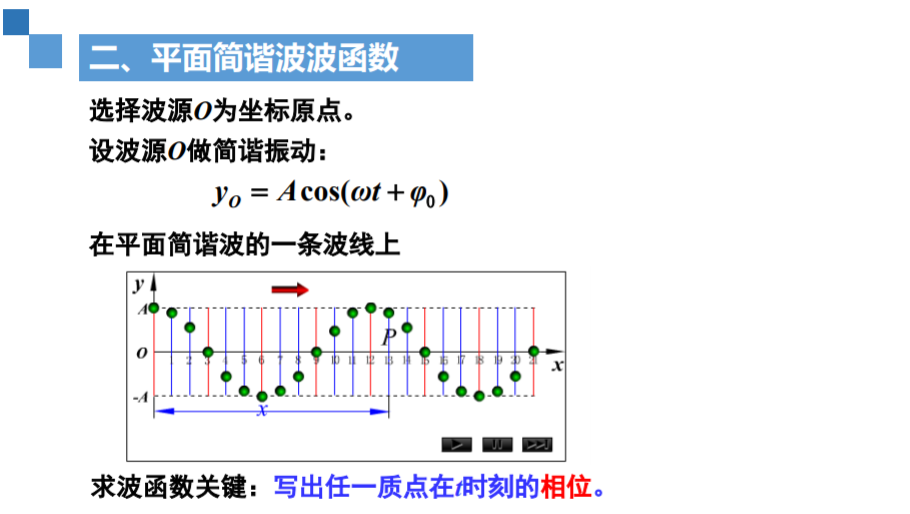
\includegraphics[width=13cm, height=8cm]{D:/UniversityNote/PhyNote/10/1001.png}
    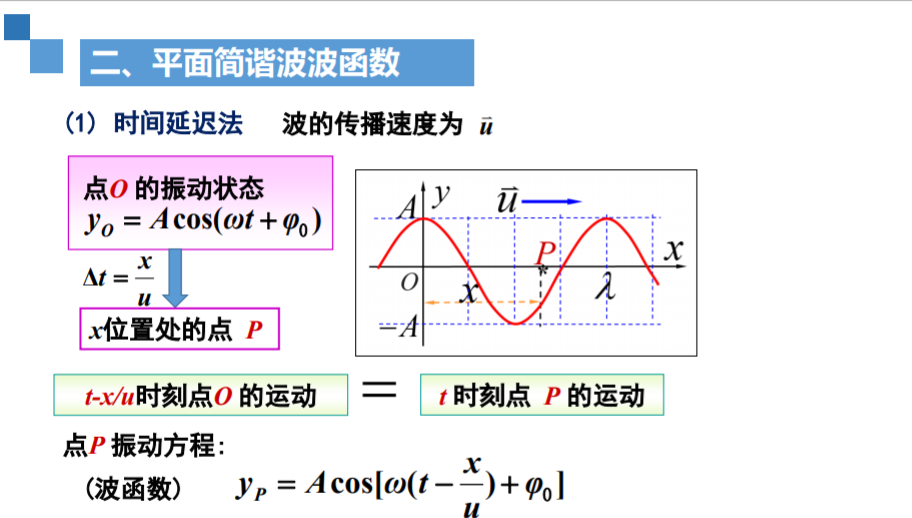
\includegraphics[width=13cm, height=8cm]{D:/UniversityNote/PhyNote/10/1002.png}
    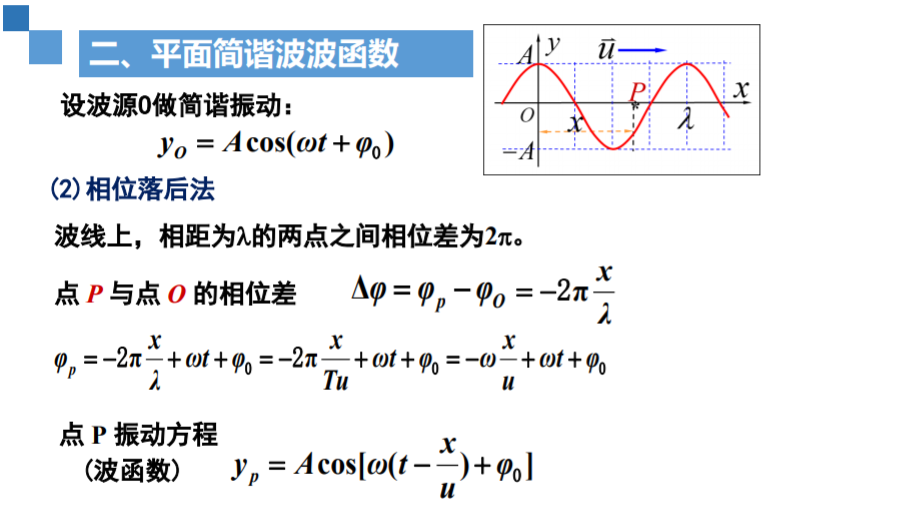
\includegraphics[width=13cm, height=8cm]{D:/UniversityNote/PhyNote/10/1003.png}
    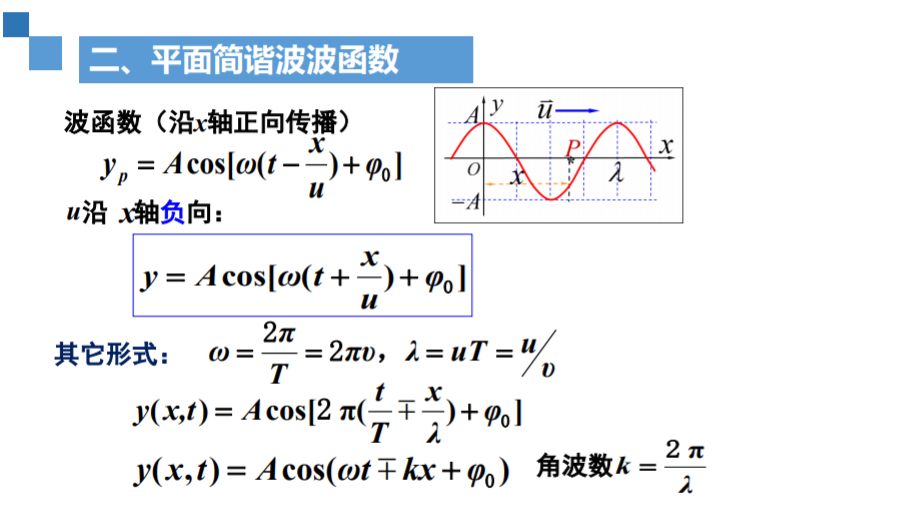
\includegraphics[width=13cm, height=8cm]{D:/UniversityNote/PhyNote/10/1004.png}
    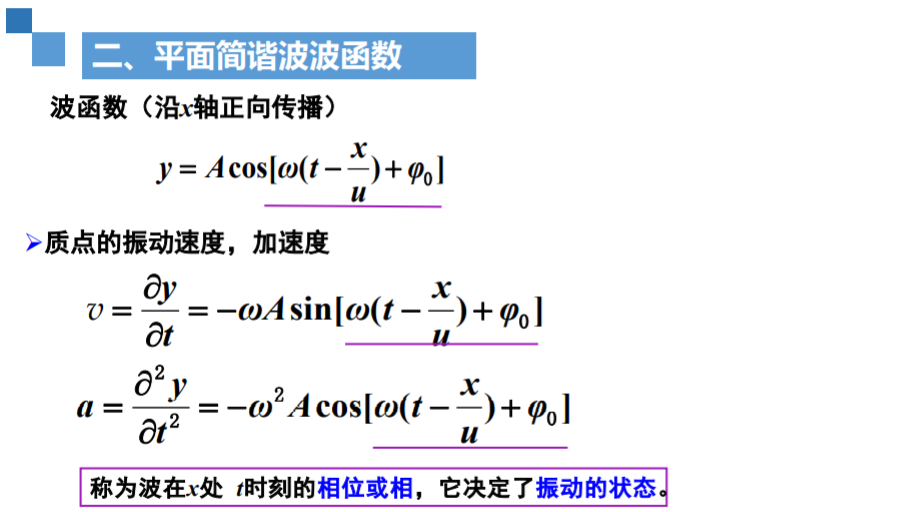
\includegraphics[width=13cm, height=8cm]{D:/UniversityNote/PhyNote/10/1005.png}

    波函数(沿x轴正向传播):$y = Acos[\omega(t - \frac{x}{u}) + \phi_0]$

    对于某一给定的相位
    \[\omega (t - \frac{x}{u}) = \mbox{常量}\phi\]

    两边对t求导可得相位的传播速度
    \[\frac{dx}{dt} = u\]

    说明波的相位的传播速度就是波的速度u,所以波速u也称为相速度,它可以超过光速

\subsection{波函数的物理意义和波动方程}

    一、波函数的物理意义
    \[y = Acos[\omega(t - \frac{x}{u} + \phi_0)] = Acos[2\pi(\frac{t}{T} - \frac{x}{\lambda}) + \phi_0]\]

    1.x固定时,表示该点的振动方程,体现波的时间周期性

    2.当t一定时,表示该时刻波线上各点相对其平衡位置的位移,体现波的空间周期性

    3.若x、t均变化,表示波形沿传播方向的运动情况(行波)

    二、波动方程
    \[y = Acos[\omega(t - \frac{x}{u} + \phi_0)]\]

    对变量二次求导
    \[\frac{\partial^2y}{\partial t^2} = -\omega^2Acos[\omega(t - \frac{x}{u} + \phi_0)]\]
    \[\frac{\partial^2y}{\partial x^2} = -\frac{\omega^2}{u^2}Acos[\omega(t - \frac{x}{u} + \phi_0)]\]

    波动微分方程
    \[\frac{\partial^2y}{\partial x^2} = \frac{1}{u^2}\frac{\partial^2y}{\partial t^2}\]

    具有普适性,即对任意一维平面波都成立

\subsection{机械波的能量}

    一、波动能量的传播

    以固体棒中传播的纵波为例分析波动能量的传播

    波函数:$y = Acos\omega(t - \frac{x}{u})$,介质密度为$\rho$

    振动动能:
    \[dW_k = \frac{1}{2}(dm)v^2 = \frac{1}{2}(\rho dV)v^2 = \frac{1}{2}\rho dVA^2\omega^2sin^2\omega(t - \frac{x}{u})\]

    弹性势能:
    \[dW_p = \frac{1}{2}k(dy)^2 = \frac{1}{2}\rho dVA^2\omega^2sin^2\omega (t - \frac{x}{u})\]

    \[dW_k = dW_p = \frac{1}{2}\rho dVA^2\omega^2sin^2\omega(t - \frac{x}{u})\]

    体积元的总机械能:
    \[dW = dW_k + dW_p = \rho dVA^2\omega^2sin^2\omega(t - \frac{x}{u})\]

    1. 传播的媒质中,任一质元的动能、势能、总机械能均作同相位的周期性变化

    \;\;平衡位置时,三者均最大

    \;\;位移最大时,三者均为零

    2. 传播的媒质中,任一质元不断地传播能量,机械能不守恒

    3. 传播的媒质中,质元做的是受迫振动,而非简谐振动

    能量密度:单位体积介质中的波动能量
    \[w = \frac{dW}{dV} = \rho A^2\omega^2sin^2\omega(t - \frac{x}{u})\]

    平均能量密度:能量密度在一个周期内的平均值
    \[\overline{w} = \frac{1}{T}\int_0^Twdt = \frac{1}{2}\rho\omega^2 A^2\]

    能流:单位时间通过介质中某一面积的能量
    \[p = \frac{wSudt}{dt} = wSu\]

    平均能流:能流在一个周期内的时间平均值
    \[\overline{P} = \overline{w}uS\]

    平均能流密度(波的强度)I:通过与波传播方向垂直的单位
    面积的平均能流
    \[I = \frac{\overline{P}}{S} = \overline{w}u\Rightarrow I = \frac{1}{2}\rho A^2\omega^2u\]

\subsection{波的衍射\;\;惠更斯原理}

    一、波的衍射

    波传播遇到障碍物时,波的传播方向偏离原来直线传播方向的现象称为衍射。一切波动都具有衍射现象,衍射是波动的直接证据之一

    衍射特点:障碍物(受限)的尺度与波长相接近时,能够观察到明显的衍射现象

    二、惠更斯原理

    在波的传播过程中,波前上每一点都可以看作是发射子波的波源,而在其后的任意时刻,这些子波的包络面就是新的波前

    原理依据: 
    
    \;\;1. 波动在介质是逐点传播;

    \;\;2. 波动是振动状态的传播。同一波前上所有子波源的振动状态完全相同,因此,其后任意时刻各子波都具有相同的相位  

    衍射的实质是波面破损或畸变

    惠更斯原理的局限性:无法说明子波强度的分布和子波不向后传播的问题

    三、惠更斯——菲涅耳原理

    波前(波阵面)上每个面元都可以看成是发出球面子波的波源;各子波在空间某点的相干叠加,就决定了该点波的强度。原理的核心是子波相干叠加

\subsection{波的反射和折射}

    一、反射定律

    1.反射线、入射线和界面的法线在同一平面内

    2.$i = i^{'}$

    二、折射定律

    1.折射线、入射线和界面的法线在同一平面内

    2.$\frac{sin i}{sin r} = \frac{u_1}{u_2}$

\subsection{波的干涉}

    一、波的叠加原理

    几列波相遇之后,仍然保持它们各自原有的特征(频率、波长、振幅、振动方向等)不变,并按照原来的方向继续前进,好象没有遇到过其他波一样。在相遇区域内任一点的振动,为各列波单独存在时在该点所引起的振动位移的矢量和。仅在波动方程为线性方程(波强不太大)时成立

    二、波的干涉

    两列相干波相遇时,使某些地方振动始终加强,而使另一些地方振动始终减弱的现象,称为波的干涉现象。(波强的非均匀稳定分布)

    相干波的条件:

    \;\;1.频率相同

    \;\;2.振动方向平行或同一方向有分量

    \;\;3.相位相同或相位差恒定
    \[A = \sqrt{A_1^2 = A_2^2+ 2A_1A_2cos\Delta\phi}\;\;\Delta\phi = \phi_2 - \phi_1 - \frac{2\pi}{\lambda}\delta\]

    波程差:$\delta = r_2 - r_1$

    $\delta = \pm k\lambda\;\;k = 0, 1, 2,\dots\;\;A = A_1 + A_2$\;\;振动始终加强

    $\delta = \pm(k + \frac{1}{2})\lambda\;\;k = 0, 1, 2,\dots\;\;A = \vert A_1 - A_2\lvert $\;\;振动始终减弱

    $\delta = \mbox{其他}\;\;\vert A_1 - A_2 \lvert < A < A_1 + A_2$

\subsection{半波损失}

    一、驻波的产生

    振幅都相同的两列相干波,在同一直线上沿相反方向传播时,某些点的合振幅始终为零(波节),某些点的合振幅始终最大(波腹),这种特殊的干涉现象就称为驻波

    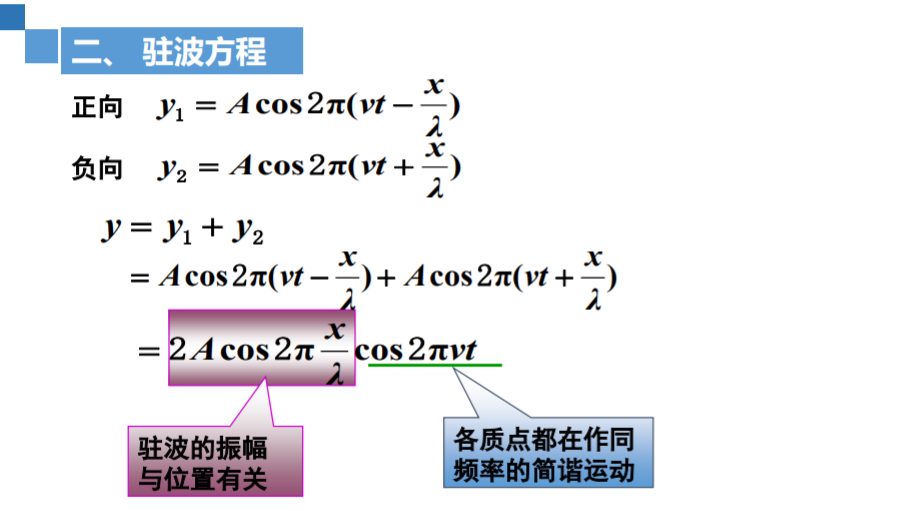
\includegraphics[width=13cm, height=8cm]{D:/UniversityNote/PhyNote/10/1006.png}
    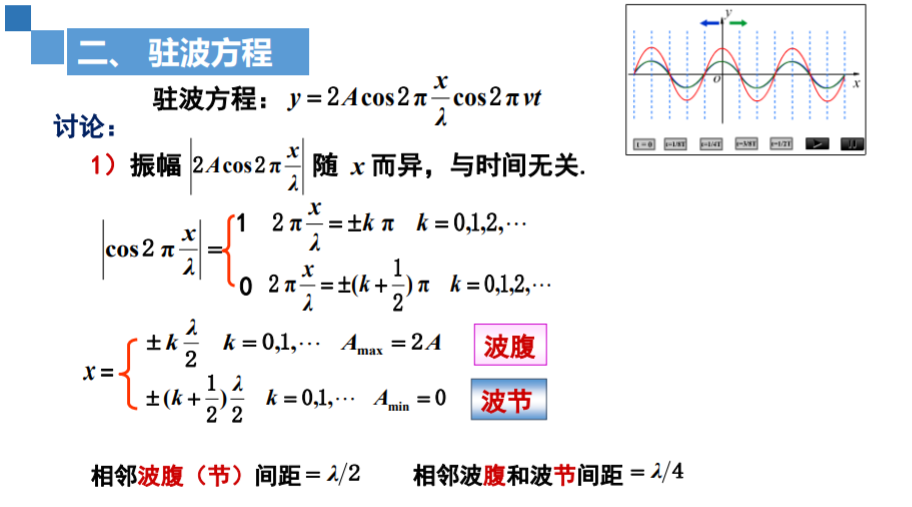
\includegraphics[width=13cm, height=8cm]{D:/UniversityNote/PhyNote/10/1007.png}
    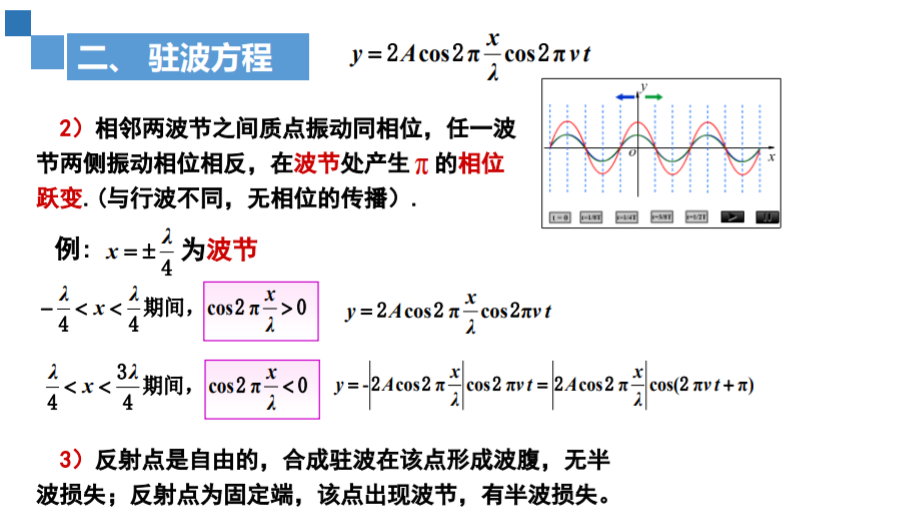
\includegraphics[width=13cm, height=8cm]{D:/UniversityNote/PhyNote/10/1008.png}
    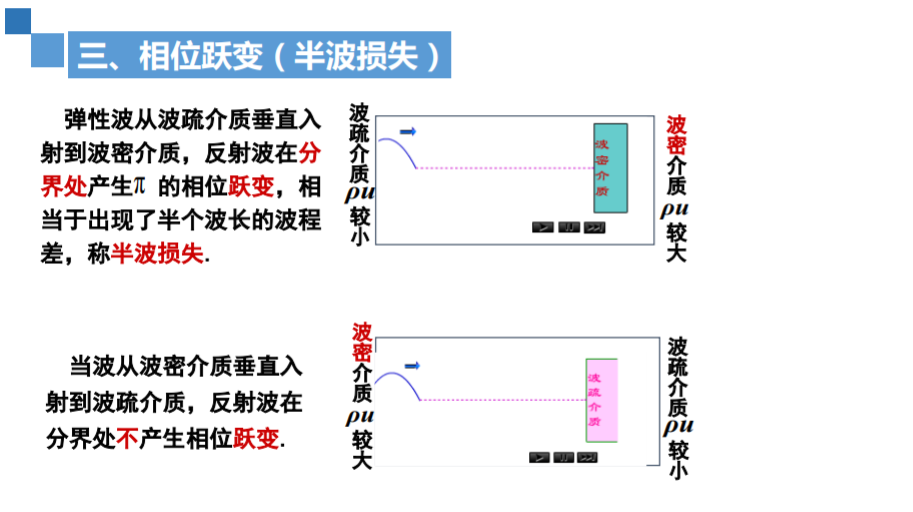
\includegraphics[width=13cm, height=8cm]{D:/UniversityNote/PhyNote/10/1009.png}
    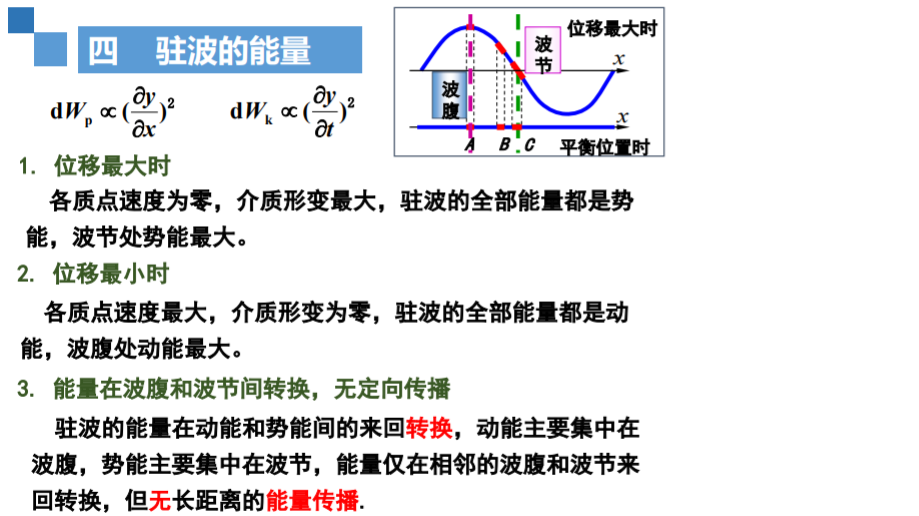
\includegraphics[width=13cm, height=8cm]{D:/UniversityNote/PhyNote/10/1010.png}

\subsection{多普勒效应}

    1. 多普勒效应定义
    
    若波源或观察者,或两者同时相对介质运动,则观察者接收到的的频率和波源的振动频率不同的现象,称为多普勒效应

    2. 机械波的多普勒效应
    \[\nu^{'} = \frac{u\pm v_0cos\beta}{u\pm v_s cos\alpha}\nu\]
    其中:
    
    $\nu$波源振动的频率;$\nu^{'}$:探测器探测的频率;$u$:波相对于介质的速度;$v_0$:探测器相对于介质的速度;$v_s$:波源相对于介质的速度


    3. 电磁波的多普勒效应
    光源和接收器在同一直线上运动时,考虑相对论效应:
    \[\nu^{'} = \sqrt{\frac{c + v}{c - v}\nu}\]

    v是光源和接收器的相对运动速度

    两者相向运动时,接收波长变短,这种现象称为“紫移”。光源和接收器相背运动时,接收波长变长,这种现象称为“红移”
    
\end{document}